\section{Modelos de Casos de Uso}
\subsection{Modelo de Casos de Uso de alto nível}

Diagrama geral de Use Cases

\begin{comment}
\begin{figure}[!htb]
	\centering
	\includegraphics[scale=0.85]{images/diagramaGeralDeUseCase}
	\caption {Diagrama geral de \emph{Use Cases} do produto}
\end{figure}
\end{comment}


\subsection{Modelos de Casos de Uso detalhado}


\subsubsection{\textbf{1 - HoneyPot}}

Tal como apresentado no diagrama abaixo, o QEMU é capaz de identificar system calls do guest OS mais seu contexto. Após detectar uma chamada este
actualiza a Base de dados com essa informação. O QEMU pode também copiar qualquer ficheiro do guest OS para o Host OS ou para outro ponto remoto.
Mais ainda o QEMU é capaz de capturar uma sequência de capturas de ecrã do que se passa no guest, criando assim um ficheiro em formato vídeo para, 
mais tarde o utilizador poder ver.

\begin{comment}
Qualquer utilizador do produto poderá efectuar uma simulação de seguro automóvel. No entanto, cada utlizador terá acesso a pequenas funcionalidades diferentes dependendo do tipo de utiliador em que se insere (registado ou não, mediador, etc). Aqui apresentaremos o fluxo normal deste \emph{use case} para um utilizador básico, ou seja, sem qualquer tipo de privilégios. Mais à frente, na explicação dos \emph{use cases} que se seguem, abordaremos as funcionalidades extra que cada tipo de utilizador terá. 
\end{comment}

\begin{figure}[!htb]
	\centering
	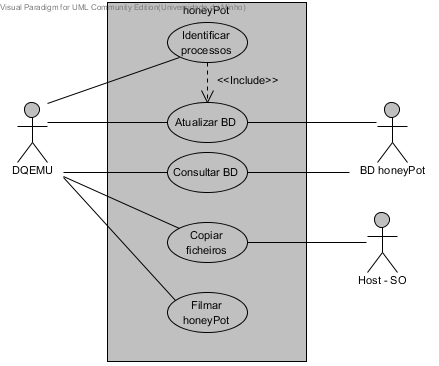
\includegraphics[scale=0.80]{images/ucs/HoneyPot}
	\caption {Diagrama de use case, parte do HoneyPot}
\end{figure}
\pagebreak




\subsubsection{\textbf{2 - Rede}}

O Delusion Collector Daemon (DCD) tem como função capturar todo o tipo de trâfego que passe pela máquina. Para isso acontecer, o DCD usa o Snort e o
Tshark (duas ferramentas de redes), para captura de trâfego e geração de alertas. Quando o DCD recolhe a informação referida, guarda-a numa 
base de dados específica. Podemos assim ver o DCD como um coletor de toda a informação que tanto o Snort como o TShark geram, passando de seguida
essa informação para uma bd.

\begin{comment}
A realização de seguro de saúde é semelhante à automóvel, sendo que os dados a serem fornecidos são diferentes. De momento, estamos a considerar relevantes apenas o sexo e data de nascimento das pessoas seguradas, assim como o grau de parentesco entre si. Temos portanto em conta que podem ser seguradas várias pessoas e que o tomador não é necessariamente uma delas.
\end{comment}


\begin{figure}[!htb]
	\centering
	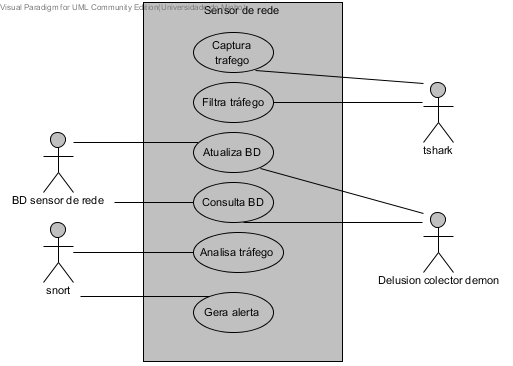
\includegraphics[scale=0.80]{images/ucs/Rede}
	\caption {Diagrama de use case, parte da Rede}
\end{figure}
\pagebreak




\subsubsection{\textbf{3 - Visualizador}}

Através do visualizador, um utilizador normal pode ver toda a informação gerada pelo sistema. Mais, pode ver essa informação filtrada, bem como,
representada a seu gosto. Podendo para isso aplicar um critério à sua escolha para o filtro, ou, um gráfico à sua escolha para a representação.
Além disso o utilizador pode ver no visualizador todos os alertas gerados pelo sistema. 
Adicionalmente o utilizador pode configurar os parâmetros de rede e instâncias do HoneyPot (por exemplo: Vulnerabilidades, tamanho de memória RAM,
Sistema operativo \ldots).
O Administrador tem mais algumas opções disponíveis que o utilizador normal. Este pode criar ou remover utilizadores e pode gerir as permissões de
cada utilizador (por exemplo: acesso a configurações de honeypot, tipos de alertas que pode ver \ldots).

\begin{comment}
É possível incluir vários produtos numa mesma simulação. Para o efeito, o utilizador procederá como numa simulação normal, preenchendo os dados correspondentes ao primeiro produto a simular. Terminada esta simulação, é apresentada ao utilizador a opção "acrescentar novo produto (simulação multi-produto)" que, quando seleccionada, agrega a presente simulação à carteira de simulações e apresenta a possibilidade de realização de simulação de um novo produto. 

Repetindo este processo, e quando satisfeito com o número de produtos simulados, o Utilizador solicita o cálculo do prémio conjunto, que tem em conta os descontos aplicáveis a uma simulação multi-produto.
\end{comment}


\begin{figure}[!htb]
	\centering
	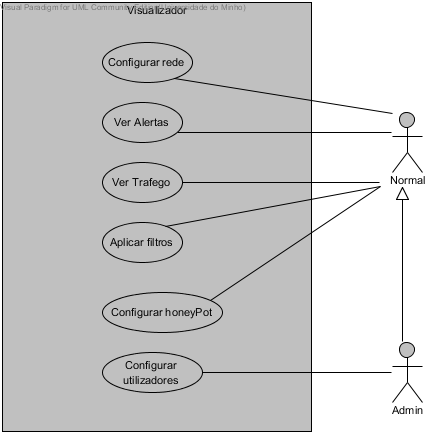
\includegraphics[scale=0.80]{images/ucs/Visualizador}
	\caption {Diagrama de use case, parte da Rede}
\end{figure}
\pagebreak






\subsubsection{\textbf{4 - Configuração HoneyPot}}

Detalhando mais os tipos de configurações que um utilizador pode fazer. Tal como já foi dito, este pode indicar o SO que quer que a máquina corra, 
pode também indicar os serviços activos e suas respectivas vulnerabilidades. Importante referir que na escolha do SO, o utilizador pode indicar os 
parâmetros de hardware da máquina.

\begin{comment}
A cada utilizador registado com simulações guardadas será dada a possibilidade de pesquisar pelas mesmas. Tal significa filtrar as simulações guardadas por produto, valor do prémio, etc. O mediador poderá também pesquisar as simulações dos seus clientes. O sistema permite também a consulta das simulações pesquisadas.
\end{comment}

\begin{figure}[!htb]
	\centering
	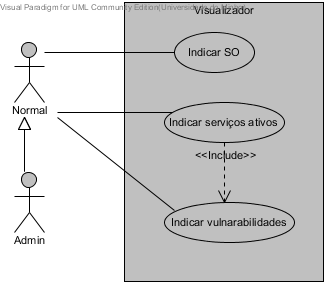
\includegraphics[scale=0.80]{images/ucs/ConfHoneyPot}
	\caption {Diagrama de use case, configuração HoneyPot}
\end{figure}
\pagebreak

\subsubsection{\textbf{5 - Configuração Rede}}

Mais uma vez, detalhando o que o utilizador pode configurar na rede. Este pode configurar a firewall (Iptables), tal como portas a bloquear, ou gamas
de ip's a bloquear. Pode configurar o Snort e o TShark para o tipo de capturas de trâfego e gerações de alertas pretendidos.

\begin{comment}
A cada utilizador registado com simulações guardadas será dada a possibilidade de pesquisar pelas mesmas. Tal significa filtrar as simulações guardadas por produto, valor do prémio, etc. O mediador poderá também pesquisar as simulações dos seus clientes. O sistema permite também a consulta das simulações pesquisadas.
\end{comment}

\begin{figure}[!htb]
	\centering
	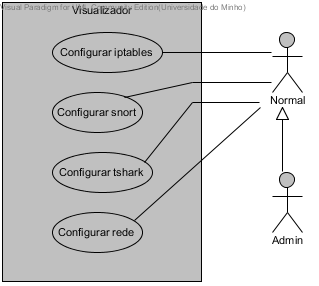
\includegraphics[scale=0.80]{images/ucs/ConfRede}
	\caption {Diagrama de use case, configuração Rede}
\end{figure}
\pagebreak

\subsubsection{\textbf{6 - Configuração Utilizadores}}

Tal como já foi dito, o administrador e só o administrador pode criar e remover utilizadores, bem como, gerir o seu perfil. Dentro do perfil este
pode configurar as permissões de cada utilizador, password de acesso entre outros.

\begin{comment}
A cada utilizador registado com simulações guardadas será dada a possibilidade de pesquisar pelas mesmas. Tal significa filtrar as simulações guardadas por produto, valor do prémio, etc. O mediador poderá também pesquisar as simulações dos seus clientes. O sistema permite também a consulta das simulações pesquisadas.
\end{comment}

\begin{figure}[!htb]
	\centering
	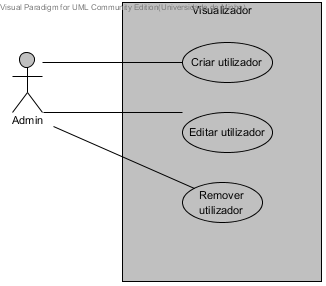
\includegraphics[scale=0.80]{images/ucs/ConfUtilizadores}
	\caption {Diagrama de use case, configuração Utilizadores}
\end{figure}
\pagebreak

